%  Typ dokumentu - článek, prezentace aj.
\documentclass[english]{article}

%  Nastaví vstupní a výstupní kódování znaků (encoding) a lokalizace
\usepackage[T1]{fontenc}
\usepackage[utf8]{inputenc}
\usepackage[english,czech]{babel}
\usepackage{icomma}
\usepackage{lmodern}

%  Formát papíru a odsazení od jeho okrajů
\usepackage[letterpaper]{geometry}
\geometry{verbose,tmargin=1.5cm,bmargin=2cm,lmargin=2cm,rmargin=2cm}

%  Umožňuje pracovat s grafikou
\usepackage{graphicx}
\usepackage{bigstrut}

%  Automaticky odsadí i první paragraf v každé sekci
\usepackage{indentfirst}

%  Umožňuje rozdělovat obsah na více sloupců
\usepackage{multicol}

%  Umožňuje používat hypertextové odkazy, nastavuje jejich barvu a
%  vlastnosti
\usepackage[unicode]{hyperref}
\hypersetup{
colorlinks=true, citecolor=blue, filecolor=blue, linkcolor=blue,
urlcolor=blue
}

%  Umožnění odstranění italiky u jednotek
\newcommand{\unit}[1]{\mathrm{#1}}

%  Formátování stránek, empty = odstraní číslování
% \pagestyle{empty}

%  Řádkování
\linespread{1.2}

%  Lepší zobrazování matematiky (rozšíření sum o \limits atd.)
\everymath{\displaystyle}

% Umožní psát přes \mathbb{N/R/Q/..} množiny čísel
\usepackage{amssymb}

%  Velikost fontu matematických výrazů v dokumentu lze pro danou
% základního fontu dokumentu upravit pomocí:
% \DeclareMathSizes{X}{Y}{Z}{U} kde:
% X je velikost fontu v dokumentu, pro kterou se matematika upraví
% Y je standartní velikost fontu matematiky
% Z je velikost fontu zmenšených (vnořených výrazů)
% U je velikost fontu ještě více zmenšených (vnořených výrazů).
\DeclareMathSizes{10}{10.5}{9}{9}

%  Nastaví autora, název, datum, skupinu měření apod. (můj vlastní
% příkaz, umožní znovu-použití v dokumentu)
\newcommand{\Author}{David Roesel}
\newcommand{\Coauthor}{Tereza Schönfeldová}
\newcommand{\Institute}{FJFI ČVUT v Praze}
\newcommand{\Subject}{FYZIKÁLNÍ PRAKTIKUM I}
\newcommand{\Group}{7}
\newcommand{\Circle}{ZS 5}
\newcommand{\Title}{Úloha \#11 \\Dynamika rotačního pohybu}
\newcommand{\Date}{1.11.2013}

% Začátek dokumentu - Formátování na výstup
\begin{document}

% Interní proměnné, možno zobrazovat u prezentací, používají se při
% generování pomocí \titlepage apod.
\author{\Author}
\title{\Title}
\date{\Date}

%  Lokalizace některých názvů do češtiny
\renewcommand{\figurename}{Obr.}
\renewcommand{\tablename}{Tab.}
\renewcommand{\refname}{Reference}

% --- Hlavička dokumentu -----------------------------------------------

\setlength{\parindent}{0cm}
\begin{multicols}{2}
\textbf{\Subject \\
        \Institute \\[0.1cm]
%\large  \Title \\[0.5cm]
\Title \\[0.5cm]
}
\begin{tabular}{rlrl}
\large Datum měření: & \Date & \large Skupina: & \Group \\
\large Jméno: & \Author & \large Kroužek:  & \Circle\\
\large Spolupracovala: & \Coauthor &\large Klasifikace:\\
\end{tabular}

\begin{flushright}

\includegraphics[scale=0.28]{../../_meta/fjfi_standart.pdf}
\hspace{0.2cm}
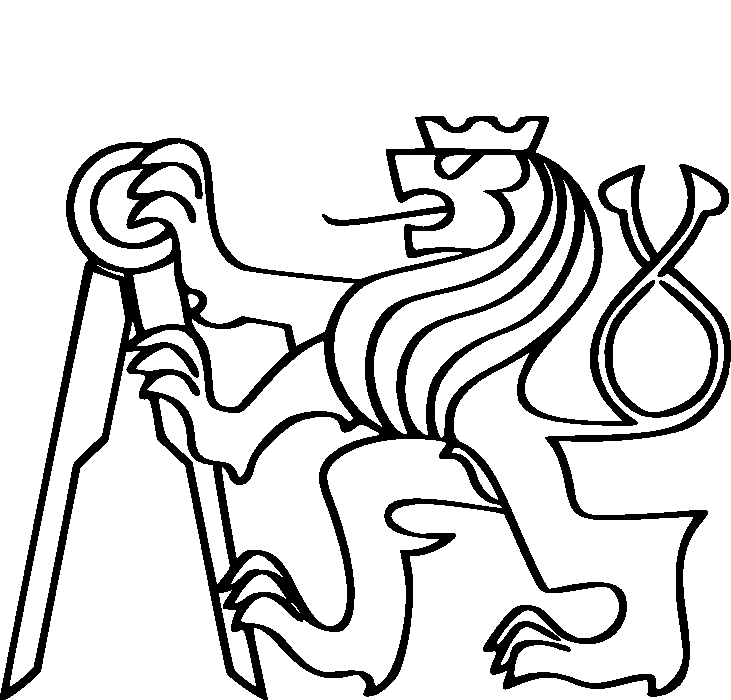
\includegraphics[scale=0.28]{../../_meta/cvut_standart.pdf}
\end{flushright}
\end{multicols}
\hrule
\vspace{0.5cm}

% ----------------------------------------------------------------------


% --- Tělo dokumentu ---------------------------------------------------
\setlength{\parindent}{0.5cm}

\section{Pracovní úkoly}
	\begin{enumerate}
	\item V domácí přípravě odvoďte vzorec pro výpočet momentu setrvačnosti válce a dutého válce. Vyjděte z definice a odvoďte vztahy (\ref{eq:disk_teo}) a (\ref{eq:prsten_teo}).
	\item Změřte momenty setrvačnosti přiložených rotačních objektů experimentálně a porovnejte je s hodnotami z teoretických vzorců. Měření proveďte alespoň pětkrát. Použijte disk, disk + prstenec a pomocí nich stanovte moment setrvačnosti samotného prstence.
	\item Změřte moment setrvačnosti disku umístěného na dráze mimo osu rotace a pomocí výsledku z předchozího úkolu ověřte platnost Steinerovy věty.
	\item Ověřte zákon zachování momentu hybnosti. Do protokolu přiložte graf závislosti úhlové rychlosti rotace na čase.
	\item Změřte rychlost precese gyroskopu jak přímo senzorem, tak i nepřímo z měření rychlosti rotace disku. Měření proveďte alespoň pětkrát.
	\end{enumerate}

\section{Vypracování}

\subsection{Použité přístroje}
	"A"\ base rotational adapter PASCO CI-6690, přídavný disk a prstenec, rotační dráha se dvěma závažími, Gyroskop PASCO ME-8960, Přídavný disk gyroskopu ME-8961, dva rotační senzory PASCO PS-2120, USB link PASCO 2100, PC, program Datastudio, nit, posuvné měřítko, stojan s kladkou, milimetrové měřítko, svinovací metr, váhy.

\subsection{Teoretický úvod}
\subsubsection{Moment setrvačnosti}
Rotační vlastnosti tělesa popisujeme jeho momentem setrvačnosti $I$. Jedná se o symetrický tenzor, který můžeme vyjádřit pomocí tří diagonálních složek - hlavních momentů setrvačnosti. Pro symetrické objekty se vztah ještě zjednoduší. Moment setrvačnosti je pro homogenní těleso o hustotě $\varrho$ definován následujícím vztahem

\begin{equation}
I = \varrho \int_{V} r^2 \mathrm{d}V. 
\end{equation}

Z něj můžeme integrací odvodit vztah pro rotující disk 

\begin{equation}
I = \int_{V} \varrho r^2 \mathrm{d}V = 
\varrho \int_{0}^{h}\int_{0}^{R}\int_{0}^{2 \pi} r^3 \mathrm{d}z \mathrm{d}r \mathrm{d}\varphi = 
\frac{M}{2}\frac{h \pi}{V} R^4 = \frac{1}{2} M R^2,
\label{eq:disk_teo}
\end{equation}
kde $R$ je poloměr, $M$ hmotnost daného tělesa, $V = \pi R^2 h$ objem válce a $\varrho = M/V$ jeho hustota.

Stejně tak pro rotující prstenec

\begin{equation}
I = \int_{V} \varrho r^2 \mathrm{d}V = 
\varrho \int_{0}^{h}\int_{R_1}^{R_2}\int_{0}^{2 \pi} r^3 \mathrm{d}z \mathrm{d}r \mathrm{d}\varphi = 
\frac{M}{2} \frac{h \pi}{V} (R_2^4 - R_1^4)  = \frac{1}{2} M (R_2^2 + R_1^2),
\label{eq:prsten_teo}
\end{equation}
kde $R_1$ je vnitřní poloměr, $R_2$ vnější poloměr, $M$ hmotnost daného tělesa, $V = \pi (R_2^2-R_1^2) h$ objem válce a $\varrho = M/V$ jeho hustota.

Zachováme-li osu rotace, platí také další významná vlastnost momentu setrvačnosti - \emph{aditivita}.

Experimentální stanovení momentu setrvačnosti provádíme podle Obr. \ref{fig:s_aparatura_moment}. Bude-li na kotouč působit konstantní síla prostřednictvím kladky, získá úhlové zrychlení $\varepsilon$ a platí
\begin{equation}
N = I \varepsilon.
\end{equation}
Z našeho uspořádání je vidět, že je moment síly $N$ popsán vztahem
\begin{equation}
N = r F = r m ( g - a ) = r m ( g - \varepsilon r ),
\end{equation}
kde $r$ je poloměr roztáčené kladky, $m$ je hmotnost závaží, $a$ jeho zrychlení, $F$ síla napínající vlákno a $g$ tíhové zrychlení.

Tedy výsledný vzorec je
\begin{equation}\label{eq:moment_setrvacnosti_final}
I = m r ( \frac{g}{\varepsilon} - r ).
\end{equation}

\subsubsection{Steinerova věta}

Pokud těleso nerotuje kolem osy procházející těžištěm, dá se použít pro výpočet momentu setrvačnosti Steinerova věta
\begin{equation}\label{eq:steinerova_veta}
I = I_0 + Ma^2,
\end{equation}
kde $I_0$ je moment setrvačnosti vzhledem k ose procházející těžištěm a $a$ je kolmá vzdálenost těžiště od osy rotace.

\subsubsection{Zákon zachování momentu hybnosti}
Moment hybnosti definujeme jako
\begin{equation}\label{eq:moment_hybnosti_final}
L = I \omega
\end{equation}
a pokud na soustavu nepůsobí vnější momenty síly, tak se zachovává. Změníme-li tedy moment setrvačnosti změnou distribuce hmotnosti ve studovaném tělese, musí se změnit rychlost rotace. Pro přesné ověření tohoto zákona je třeba změnu provádět okamžitě.

\subsubsection{Precese gyroskopu}
Rychlost precese gyroskopu měříme na horizontálním setrvačníku upevněném na pohyblivé ose. Na počátku je gyroskop vyvážen v základní poloze. Tím, že umístíme závaží o hmotnosti $m_p$ do vzdálenosti $d$ od osy gyroskopu, začne působit moment síly, který setrvačník vyvede z rovnováhy. Pro tento moment síly definovaný jako $N=m_pgd$ platí 
\begin{equation}
N = \frac{\mathrm{d}L}{\mathrm{d}t},
\end{equation}
kde $L$ je moment setrvačnosti disku, který se točí s úhlovou rychlostí $\omega$. Pro malé výchylky $\mathrm{d} \phi$ platí podle Obr. \ref{fig:s_aparatura_gyro} vztah
\begin{equation}
\mathrm{d}L = L \mathrm{d}\phi
\end{equation}
a z toho
\begin{equation}
N = L \frac{\mathrm{d}\phi}{\mathrm{d}t} = L \Omega,
\end{equation}
kde $\Omega$ je hledaná precesní rychlost. Vzorec pro teoretický výpočet úhlové rychlosti precese je tedy
\begin{equation} \label{eq:precese_final}
\Omega = \frac{m_p g d}{I \omega}.
\end{equation}
Měřené úhlové rychlosti je pak potřeba převést pomocí vzorce
 \begin{equation}
 \omega = \frac{r_s}{r} \omega_s,
 \label{eq:prevody}
 \end{equation}
 kde $\omega_s$ je úhlová rychlost naměřená senzorem, $r_s$ poloměr kladky senzoru a $r$ poloměr kladky na měřené ose.
		
\subsection{Postup měření}
	\subsubsection{Momenty setrvačnosti}
	Aparaturu jsme sestavili podle Obr. \ref{fig:s_aparatura_moment} a zvážili všechny disky a závaží pro teoretické výpočty. Pak jsme měřili podle následujícího postupu momenty setrvačnosti pro disk a disk s prstencem.
	\begin{enumerate}
		\item Pokusíme se soustavu vyrovnat tak, aby byla podstava vodorovně.
		\item Namotáme nit na kladku ze správné strany a zavěsíme na ni závaží.
		\item Při zapnutém zaznamenávání necháme závaží volně padat k zemi a roztáčet soustavu.
		\item Z grafu odečteme hodnotu úhlového zrychlení pomocí lineárního proložení.
	\end{enumerate}
	
	\subsubsection{Steinerova věta}
		Aparaturu jsme nechali sestavenou stejně jako při předchozí úloze, jen místo disku jsme ze shora upevnili rotační dráhu. Na ni jsme pomocí nástavce ve vzdálenosti co nejbližší jejímu středu přidělali již proměřovaný disk. Pomocí postupu z předchozí úlohy jsme pak změřili momenty setrvačnosti dráhy s diskem a dráhy pouze s nástavcem. 

	\subsubsection{Zákon zachování momentu hybnosti}
	Nadále jsme používali rotační dráhu, ale umístili jsme na ni zarážky a dvě závaží, každé z nich jedním směrem od osy otáčení a obě do stejné vzdálenosti. Vnitřní zarážky byly umístěny přibližně do vzdálenosti $8,5$ cm, vnější pak přibližně $17$ cm daleko. Obě závaží byly spojeny provázkem, který byl provléknutý osou stojanu. Zatáhnutím za provázek se tak dalo měnit rozmístění hmotnosti a tím i moment setrvačnosti soustavy. Při vlastním měření jsme postupovali podle následujících kroků:
	\begin{enumerate}
		\item Závaží umístíme k vnějším zarážkám.
		\item Roztočíme dráhu a začneme zaznamenávat data.
		\item Chvíli měříme aktuální úhlovou rychlost.
		\item Prudce zatáhneme za provázek a závaží tak dostaneme až ke vnitřním zarážkám.
		\item Provázek držíme napnutý a chvíli měříme novou úhlovou rychlost.
		\item Vypneme zaznamenávání dat, zastavíme rotaci dráhy a vrátíme závaží na původní místo.
	\end{enumerate}
	
	\subsubsection{Precese gyroskopu}
	Sestavení aparatury je patrné na Obr. \ref{fig:s_aparatura_gyro}. Před vlastním měřením jsme zvážili závaží, změřili poloměry všech převodů na aparatuře a pomocí tří závaží vyvážili gyroskop. Na určené místo za rotační disk jsme poté umístili závaží a změřili jeho vzdálenost od osy gyroskopu, čímž jsme konkrétním způsobem narušili rovnováhu a mohli tak sledovat precesi. Vlastní měření jsme prováděli podle následujícího postupu:
	\begin{enumerate}
		\item Pevně držíme podstavu, aby při roztáčení zůstala na místě.
		\item Osu kotouče chytíme do jedné ruky a druhou roztočíme kotouč.
		\item Pustíme osu a začneme zaznamenávat hodnoty precesního pohybu a úhlovou rychlost otáčení disku.
		\item Zastavíme záznam hodnot a za držení osy zastavíme kotouč.
	\end{enumerate}
	
\subsection{Naměřené hodnoty}
		
	\subsubsection{Momenty setrvačnosti}
		Hmotnost samotného disku jsme změřili na $m_d=(1,407\pm0,001)$ kg a jeho poloměr pak na $r_d=(11,45\pm0,05)$ cm. Moment setrvačnosti disku jsme tak podle (\ref{eq:disk_teo}) určili teoreticky na 
		\begin{equation}
			I_{dt} = (9,22\pm0,08) \cdot \unit{10^{-3} \cdot kg \cdot m^3}.
		\end{equation}

		Hmotnost prstence jsme změřili na $m_p=(1,407\pm0,001)$ kg, jeho vnitřní poloměr na $r_{p1}=(5,36\pm0,05)$ cm a jeho vnější poloměr na $r_{p2}=(6,37\pm0,05)$ cm. Moment setrvačnosti prstence jsme tak podle (\ref{eq:prsten_teo}) určili teoreticky na 
		\begin{equation}
			I_{pt} = (4,88\pm0,06) \cdot \unit{10^{-3} \cdot kg \cdot m^3}.
		\end{equation}
		
		Naměřené hodnoty pro experimentální určení momentů setrvačnosti disku a disku s prstencem jsou v Tab. \ref{tab:moment_disk} a \ref{tab:moment_disk_a_prst}. Hmotnost roztáčecího závaží jsme určili na $m_{sp} = (48,8\pm0,1)$ g, poloměr roztáčecí kladky pak na $r_m = (1,48\pm0,05)$ cm.  Moment setrvačnosti disku a disku s prstencem jsme tedy určili podle (\ref{eq:moment_setrvacnosti_final}) na
		\begin{equation}
			I_{d+p} = (16,0\pm0,5) \cdot \unit{10^{-3} \cdot kg \cdot m^3}, \qquad 
			I_{d} = (10,0\pm0,3) \cdot \unit{10^{-3} \cdot kg \cdot m^3}
		\end{equation}
		a z toho pak díky aditivitě moment setrvačnosti samotného prstence		
		\begin{equation}
			I_{p} = (6,0\pm0,6) \cdot \unit{10^{-3} \cdot kg \cdot m^3}.
		\end{equation}
		
		Chyby přímého měření momentů setrvačnosti jsme v tomto i dalších úkolech určovali podle (\ref{eq:vazeny_prumer}), u ostatních výpočtů pak podle (\ref{eq:chyba_neprime_mereni}).
				
	\subsubsection{Steinerova věta}
		Hmotnost i moment setrvačnosti samotného disku jsme změřili v předchozí úloze, vzdálenost disku od osy otáčení jsme určili na $a=(12,5\pm0,1)$ cm. Z toho nám podle (\ref{eq:steinerova_veta}) vyšel teoretický moment setrvačnosti disku ve vzdálenosti $a$ jako 
		\begin{equation}
			I_{st} = (31,2\pm0,4) \cdot \unit{10^{-3} \cdot kg \cdot m^3}.
		\end{equation}
		
		Naměřené hodnoty pro experimentální určení momentů setrvačnosti samotné dráhy s nástavcem a dráhy po přidání disku jsou v Tab. \ref{tab:steiner_draha} a \ref{tab:steiner_draha_a_disk}. Moment setrvačnosti samotné dráhy s nástavcem a dráhy s přidaným diskem jsme tedy určili pomocí (\ref{eq:moment_setrvacnosti_final}) na
		\begin{equation}
			I_{dr+d} = (49\pm2) \cdot \unit{10^{-3} \cdot kg \cdot m^3}, \qquad 
			I_{dr} = (14,6\pm0,05) \cdot \unit{10^{-3} \cdot kg \cdot m^3}
		\end{equation}
		a z toho pak díky aditivitě moment setrvačnosti samotného disku ve vzdálenosti $a$		
		\begin{equation}
			I_{s} = (34\pm2) \cdot \unit{10^{-3} \cdot kg \cdot m^3}.
		\end{equation}		
		
	\subsubsection{Zákon zachování momentu hybnosti}
		Naměřené hodnoty pro experimentální určení momentů setrvačnosti obou poloh závaží jsou v Tab. \ref{tab:zzmh_zavazi_odsebe} a \ref{tab:zzmh_zavazi_usebe}. Moment setrvačnosti dráhy při obou polohách jsme tedy určili pomocí (\ref{eq:moment_setrvacnosti_final}) na
		\begin{equation}
			I_{min} = (18,8\pm0,6) \cdot \unit{10^{-3} \cdot kg \cdot m^3}, 
		\end{equation}	
		\begin{equation}
			I_{max} = (32\pm1) \cdot \unit{10^{-3} \cdot kg \cdot m^3} 
		\end{equation}	
		
		Parametry fitů naměřených hodnot jsou uvedeny v Tab. \ref{tab:zzmh}, průběh jednoho měření vyexportovaný z programu \emph{DataStudio} je vidět na Obr. \ref{fig:g_zzmh}, poměry momentů hybností naměřených před a po změně rozložení hmotnosti jsou vyneseny v Tab. \ref{tab:zzmh_k} a finální poměr momentů hybností nám z nich vyšel
		\begin{equation}
			k_f = (0,99\pm0,02), 
		\end{equation}			
		přičemž chybu jednotlivých $k$ jsme určili pomocí (\ref{eq:chyba_neprime_mereni}) a celkového $k_f$ potom pomocí (\ref{eq:vazeny_prumer}).
		
	\subsubsection{Precese gyroskopu}
		Odečtené hodnoty fitů precese gyroskopu a úhlové rychlosti rotace disku jsou vyneseny v Tab. \ref{tab:gyro_precese_fit} a \ref{tab:gyro_rychlost_fit}. Hodnoty úhlových rychlostí spočítané z precese dosazením do rovnice lineárního fitu jsou v Tab. \ref{tab:gyro_precese_data}. Hodnoty spočítané teoreticky pomocí (\ref{eq:precese_final}) jsou pak v Tab. \ref{tab:gyro_rychlost_data}. K výpočtu byl potřeba moment setrvačnosti disku gyroskopu, který jsme pro hmotnost $m = (1,712\pm0,001)$ kg určili pomocí (\ref{eq:disk_teo}) na 
		
		\begin{equation}
			I_{g} = (13,9\pm0,1) \cdot \unit{10^{-3} \cdot kg \cdot m^3}.
		\end{equation}		
		
		Převody jsme počítali pomocí vzorce (\ref{eq:prevody}). Poloměr kladky na ose precese jsme určili jako $r_p = (2,40\pm0,01)$ cm, poloměr kladky senzoru precese pak jako $r_{p_s} = (0,76\pm0,01)$\ cm. Poloměr kladky na ose disku jsme určili jako $r_d = (2,89\pm0,01)$ cm, poloměr kladky senzoru rychlosti disku pak jako $r_{d_s} = (2,10\pm0,1)$ cm. 
	
\subsection{Diskuse}
	\subsubsection{Momenty setrvačnosti}
		Z námi změřených hodnot byly přesnější ty teoreticky počítané, což je nejspíš způsobeno tím, že jsou zatíženy pouze chybou měření hmotnosti a poloměru tělesa, které jsou relativně malé. V experimentálně změřených hodnotách momentu setrvačnosti se navíc projevuje chyba parametru fitu a pro prstenec je chyba dokonce složením chyb dvou různých měření. Teoretické hodnoty jsou pravděpodobně blíže reálnému výsledku vzhledem k tomu, že při jejich měření nemohlo dojít k tolika systematickým chybám jako u zjišťování momentu setrvačnosti experimentálně. Výsledky by se daly zpřesnit, pokud bychom používali dokonalejší pomůcky, pečlivěji vyrovnali základnu aparatury nebo prováděli měření někde, kde budou menší vnější vlivy.
			
	\subsubsection{Steinerova věta}
		Teoreticky vypočítaná hodnota je ze stejných důvodů jako v předchozí úloze přesnější než ta experimentálně zjištěná. V tomto případě se vzhledem k nerovnoměrnému rozmístění hmotnosti mnohem víc projeví nevyrovnanost podstavy a volnost aparatury. Tyto vlivy vedou k periodicky se měnící křivce a méně přesnému lineárnímu fitu. Výsledky by se daly zpřesnit stejně jako v minulé úloze, případně by se průběh úhlové rychlosti dal proložit periodickou funkcí.
		
	\subsubsection{Zákon zachování momentu hybnosti}
		Výsledky poměrů momentů hybností relativně odpovídají předpokladům. Chyby námi změřených momentů setrvačnosti se bohužel přenášely do výpočtů momentů hybnosti. Na přesnost měření mělo také velký vliv jak dlouhý úsek dat jsme prokládali. V případě proložení menšího počtu bodů byla hodnota parametrů téměř stejná jako při proložení většího množství dat, ale chyba parametrů se často změnila až o dva řády. Za zvážení by pro budoucí zpřesnění stálo používat jinou metodu odhadu chyby. Vzhledem k teoretickému předpokladu okamžité změny rozmístění hmotnosti by se měření dalo dále zpřesnit rychlejším přesunem závaží mezi polohami. Naše výsledky mohlo také ovlivnit, že jsme měli ne úplně dobře upevněné zarážky a v jedné části experimentu jsme je museli znovu utahovat.
		
	\subsubsection{Precese gyroskopu}
		Měření rychlosti precese gyroskopu se nám nepovedlo provést příliš přesně. K nepřesnostem obou metod mohlo vést to, že jsme nedostatečně vyvážili gyroskop před vlastním měřením a že se nám nepodařilo vždy dobře uhlídat, aby kabely vedoucí k senzorům nebrzdily precesní pohyb. Těžko usuzovat, které z naměřených hodnot jsou blíže realitě, s jistotou lze však říci, že nepřímé určování úhlové rychlosti precese dávalo konzistentnější výsledky. U přímého měření docházelo k nepřesnostem z řady důvodů. V první řadě jsme prokládali periodickou funkci se značnou amplitudou a tím pádem fity nebyly zcela přesné. Za druhé jsme fitovali na relativně malých časových úsecích a mohlo dojít ke stejnému problému, jako v předchozí úloze. V neposlední řadě je třeba zmínit, že byl senzor precesního pohybu nastaven na nejmenší převod, měření jeho poloměru mělo pak větší relativní chybu a navíc bylo dost komplikované se k němu posuvným měřítkem dobře dostat. Systematická chyba tohoto měření je rozhodně větší než chyba statistická.
		
\section{Závěr}
	V domácí přípravě jsme odvodili vzorec pro výpočet momentu setrvačnosti válce a dutého válce a z nich jsme určili moment setrvačnosti disku $I_{dt} = (9,22\pm0,08) \cdot \unit{10^{-3} \cdot kg \cdot m^3}$ a prstence $I_{pt} = (4,88\pm0,06) \cdot \unit{10^{-3} \cdot kg \cdot m^3}$. Dále jsme úspěšně experimentálně určili moment setrvačnosti disku $I_{d} = (10,0\pm0,3) \cdot \unit{10^{-3} \cdot kg \cdot m^3} $ a prstence $I_{p} = (6,0\pm0,6) \cdot \unit{10^{-3} \cdot kg \cdot m^3}$.
	
	Změřili jsme moment setrvačnosti disku umístěného na dráze mimo osu rotace $I_{s} = (34\pm2) \cdot \unit{10^{-3} \cdot kg \cdot m^3}$ a ač se nám nepodařilo porovnáním s teoreticky spočítanou hodnotou $I_{st} = (31,2\pm0,4) \cdot \unit{10^{-3} \cdot kg \cdot m^3}$ úspěšně ověřit platnost Steinerovy věty, můžeme při uvažování systematických chyb konstatovat, že se nám ji nepodařilo ani vyvrátit.
	
	Měřili jsme zákon zachování momentu hybnosti za pomoci předchozích výsledků a vyšlo nám, že se poměr momentů hybnosti ve dvou fázích experimentu rovná $k_f = (0,99\pm0,02)$. Zákon jsme tímto v rámci dané chyby úspěšně ověřili.
	
	Jako poslední jsme změřili rychlost precese gyroskopu přímo senzorem i nepřímo sledováním rychlosti rotace disku. V obou případech se nám hodnoty podařilo naměřit, výsledky nepřímé metody jsou však více směrodatné a zatížené menším množstvím systematických chyb.

	
\section {Použitá literatura}
% --- Literatura a reference -------------------------------------------
\begingroup
\renewcommand{\section}[2]{}

\begin{thebibliography}{9}
\bibitem{bib:zadani} Kolektiv KF, \emph{Návod k úloze: Dynamika rotačního pohybu} [Online], [cit. \today] \newline 
http://praktikum.fjfi.cvut.cz/pluginfile.php/133/mod\_resource/content/2/11\_Dynamika\_rotacniho\_pohybu.pdf

%\bibitem{bib:navody} Kolektiv KF, \emph{Návody k přístrojům} [Online], [cit. \today] \newline http://praktikum.fjfi.cvut.cz/documents/chybynav/navody-o.pdf

\bibitem{bib:chyby} Kolektiv KF, \emph{Chyby měření} [Online], [cit. \today] \newline http://praktikum.fjfi.cvut.cz/documents/chybynav/chyby-o.pdf

\end{thebibliography}
\endgroup
% ----------------------------------------------------------------------


\part{Přílohy}

\subsection{Domácí příprava}
	Domácí příprava je přiložena k protokolu.
%\clearpage
\subsection{Statistické zpracování dat}
	Pro statistické zpracování využíváme aritmetického průměru:
	\begin{equation} \label{eq:aritmeticky_prumer}
	\overline{x} = \frac{1}{n}\sum\limits_{i=1}^{n}x_i,
	\end{equation}
	
	jehož chybu spočítáme jako 
	\begin{equation} \label{eq:chyba_aritmetickeho_prumeru}
	\sigma_0 = \sqrt{\frac{1}{n(n-1)} \sum\limits_{i=1}^{n}\left( x_i - \overline{x} \right)^2 },
	\end{equation}
	
	kde $ x_i $ jsou jednotlivé naměřené hodnoty, $ n $ je počet měření, $ \overline{x} $ aritmetický průměr a $ \sigma_0 $ jeho chyba \cite{bib:chyby}.
	
Při nepřímém měření počítáme hodnotu s chybou dle následujících vztahů:
	\begin{equation}
	u = f(x, y, z, \ldots),
	\end{equation}
	\begin{displaymath}
	x = (\overline{x} \pm \sigma_x), \qquad
	y = (\overline{y} \pm \sigma_y), \qquad
	z = (\overline{z} \pm \sigma_z), \qquad
	\ldots,
	\end{displaymath}
	
	kde $ u $ je veličina, kterou určujeme nepřímo z měřených veličin $ x, y, z, \ldots $ 
	
	Pak
	\begin{displaymath}
	\overline{u} = f(\overline{x}, \overline{y}, \overline{z}, \ldots),
	\end{displaymath}
	\begin{equation}\label{eq:chyba_neprime_mereni}
	\sigma_u = \sqrt{\left( \frac{\partial f}{\partial x} \right)^2 \sigma^2_x + \left( \frac{\partial f}{\partial y} \right)^2 \sigma^2_y + \left( \frac{\partial f}{\partial z} \right)^2 \sigma^2_z + \ldots},
	\end{equation}
	\begin{displaymath}
	u = (\overline{u} \pm \sigma_ u).
	\end{displaymath}
	
V případě, že máme několik různě přesných měření stejné veličiny, používáme vztah pro vážený průměr:
	\begin{equation} 
	\bar{x}=\frac{\sum\limits_{i=1}^{n}p_{i}x_{i}}{\sum\limits_{i=1}^{n}p_{i}},
	\end{equation}
	
	kde $\bar{x}$ je vážený průměr, $x_{i}$ jsou jednotlivá měření a pro $p_{i}$ platí
	 
	\begin{equation}
	p_{i}=\frac{1}{\sigma_{i}^{2}},
	\end{equation}
	
	kde $\sigma_{i}$ jsou jednotlivé chyby daných měření.
	 
	Celkovou chybu tedy vypočítáme ze vztahu
	\begin{equation} \label{eq:vazeny_prumer}
	\sigma_{0}=\sqrt{\frac{1}{\sum\limits_{i=1}^{n}p_{i}}}.
	\end{equation}
	
	
\clearpage
\subsection{Tabulky}

\begin{table}[h]
\catcode`\-=12 % HAX na enable cline v českym bable
\parbox{.45\linewidth}{
\centering
\begin{tabular}{|r|r|r|}
      \cline{2-3}    \multicolumn{1}{r|}{} & $\varepsilon \unit{[ rad/s^2]}$ & $\sigma_{\varepsilon}\unit{ [rad/s^2]}$ \bigstrut\\
      \cline{2-3}    \multicolumn{1}{r|}{} & 0,705 & 0,001 \bigstrut\\
      \cline{2-3}    \multicolumn{1}{r|}{} & 0,686 & 0,002 \bigstrut\\
      \cline{2-3}    \multicolumn{1}{r|}{} & 0,703 & 0,002 \bigstrut\\
      \cline{2-3}    \multicolumn{1}{r|}{} & 0,709 & 0,002 \bigstrut\\
      \cline{2-3}    \multicolumn{1}{r|}{} & 0,711 & 0,002 \bigstrut\\
      \cline{2-3}    \multicolumn{1}{r|}{} & 0,695 & 0,002 \bigstrut\\
      \cline{2-3}    \multicolumn{1}{r|}{} & 0,697 & 0,002 \bigstrut\\
      \cline{2-3}    \multicolumn{1}{r|}{} & 0,707 & 0,002 \bigstrut\\
      \cline{2-3}    \multicolumn{1}{r|}{} & 0,712 & 0,001 \bigstrut\\
      \cline{2-3}    \multicolumn{1}{r|}{} & 0,713 & 0,001 \bigstrut\\
          \hline
          $\overline{\varepsilon} \pm \sigma_{\overline{\varepsilon}}$ & 0,7060 & 0,0005 \bigstrut\\
          \hline
          \end{tabular}%
      
   
  \caption{Měření úhlového zrychlení disku; $\varepsilon$ je úhlové zrychlení, $\sigma_{\varepsilon}$ jeho chyba, $\overline{\varepsilon}$ vážený průměr, $\sigma_{\overline{\varepsilon}}$ jeho chyba.}
  \label{tab:moment_disk}%
}
\hfill
\parbox{.45\linewidth}{
\centering
    \begin{tabular}{|r|r|r|}
\cline{2-3}    \multicolumn{1}{r|}{} & $\varepsilon \unit{[ rad/s^2]}$ & $\sigma_{\varepsilon}\unit{ [rad/s^2]}$ \bigstrut\\
\cline{2-3}    \multicolumn{1}{r|}{} & 0,442 & 0,001 \bigstrut\\
\cline{2-3}    \multicolumn{1}{r|}{} & 0,441 & 0,001 \bigstrut\\
\cline{2-3}    \multicolumn{1}{r|}{} & 0,445 & 0,001 \bigstrut\\
\cline{2-3}    \multicolumn{1}{r|}{} & 0,444 & 0,001 \bigstrut\\
\cline{2-3}    \multicolumn{1}{r|}{} & 0,441 & 0,001 \bigstrut\\
\cline{2-3}    \multicolumn{1}{r|}{} & 0,446 & 0,001 \bigstrut\\
\cline{2-3}    \multicolumn{1}{r|}{} & 0,446 & 0,002 \bigstrut\\
\cline{2-3}    \multicolumn{1}{r|}{} & 0,444 & 0,001 \bigstrut\\
\cline{2-3}    \multicolumn{1}{r|}{} & 0,449 & 0,001 \bigstrut\\
\cline{2-3}    \multicolumn{1}{r|}{} & 0,440 & 0,001 \bigstrut\\
    \hline
    $\overline{\varepsilon} \pm \sigma_{\overline{\varepsilon}}$ & 0,4428 & 0,0002 \bigstrut\\
    \hline
    \end{tabular}%

      
   
  \caption{Měření úhlového zrychlení disku a prstence; $\varepsilon$ je úhlové zrychlení, $\sigma_{\varepsilon}$ jeho chyba, $\overline{\varepsilon}$ vážený průměr, $\sigma_{\overline{\varepsilon}}$ jeho chyba.}
    \label{tab:moment_disk_a_prst}%

}

\end{table}

\begin{table}[h!]
\catcode`\-=12 % HAX na enable cline v českym bable
\parbox{.45\linewidth}{
\centering
    \begin{tabular}{|r|r|r|}
\cline{2-3}    \multicolumn{1}{r|}{} & $\varepsilon \unit{[ rad/s^2]}$ & $\sigma_{\varepsilon}\unit{ [rad/s^2]}$ \bigstrut\\
\cline{2-3}    \multicolumn{1}{r|}{} & 0,489 & 0,003 \bigstrut\\
\cline{2-3}    \multicolumn{1}{r|}{} & 0,479 & 0,002 \bigstrut\\
\cline{2-3}    \multicolumn{1}{r|}{} & 0,494 & 0,003 \bigstrut\\
\cline{2-3}    \multicolumn{1}{r|}{} & 0,478 & 0,002 \bigstrut\\
\cline{2-3}    \multicolumn{1}{r|}{} & 0,495 & 0,002 \bigstrut\\
\cline{2-3}    \multicolumn{1}{r|}{} & 0,487 & 0,002 \bigstrut\\
\cline{2-3}    \multicolumn{1}{r|}{} & 0,485 & 0,002 \bigstrut\\
\cline{2-3}    \multicolumn{1}{r|}{} & 0,489 & 0,003 \bigstrut\\
\cline{2-3}    \multicolumn{1}{r|}{} & 0,485 & 0,003 \bigstrut\\
\cline{2-3}    \multicolumn{1}{r|}{} & 0,479 & 0,005 \bigstrut\\
    \hline
    $\overline{\varepsilon} \pm \sigma_{\overline{\varepsilon}}$ & 0,4868 & 0,0008 \bigstrut\\
    \hline
    \end{tabular}%

      
   
  
  \caption{Měření úhlového zrychlení samotné dráhy; $\varepsilon$ je úhlové zrychlení, $\sigma_{\varepsilon}$ jeho chyba, $\overline{\varepsilon}$ vážený průměr, $\sigma_{\overline{\varepsilon}}$ jeho chyba.}
  \label{tab:steiner_draha}

}
\hfill
\parbox{.45\linewidth}{
\centering
    \begin{tabular}{|r|r|r|}
    \cline{2-3}    \multicolumn{1}{r|}{} & $\varepsilon \unit{[ rad/s^2]}$ & $\sigma_{\varepsilon}\unit{ [rad/s^2]}$ \bigstrut\\
    \cline{2-3}    \multicolumn{1}{r|}{} & 0,14  & 0,02 \bigstrut\\
    \cline{2-3}    \multicolumn{1}{r|}{} & 0,15  & 0,02 \bigstrut\\
    \cline{2-3}    \multicolumn{1}{r|}{} & 0,15  & 0,01 \bigstrut\\
    \cline{2-3}    \multicolumn{1}{r|}{} & 0,15  & 0,01 \bigstrut\\
    \cline{2-3}    \multicolumn{1}{r|}{} & 0,14  & 0,01 \bigstrut\\
    \cline{2-3}    \multicolumn{1}{r|}{} & 0,15  & 0,02 \bigstrut\\
    \cline{2-3}    \multicolumn{1}{r|}{} & 0,15  & 0,02 \bigstrut\\
    \cline{2-3}    \multicolumn{1}{r|}{} & 0,15  & 0,01 \bigstrut\\
    \cline{2-3}    \multicolumn{1}{r|}{} & 0,14  & 0,02 \bigstrut\\
    \cline{2-3}    \multicolumn{1}{r|}{} & 0,15  & 0,01 \bigstrut\\
        \hline
        $\overline{\varepsilon} \pm \sigma_{\overline{\varepsilon}} $ & 0,145 & 0,005 \bigstrut\\
        \hline
        \end{tabular}%
    

      
   
  \caption{Měření úhlového zrychlení dráhy s diskem; $\varepsilon$ je úhlové zrychlení, $\sigma_{\varepsilon}$ jeho chyba, $\overline{\varepsilon}$ vážený průměr, $\sigma_{\overline{\varepsilon}}$ jeho chyba.}
    \label{tab:steiner_draha_a_disk}%

}

\end{table}

\begin{table}[h]
\catcode`\-=12 % HAX na enable cline v českym bable
\parbox{.45\linewidth}{
\centering
    \begin{tabular}{|r|r|r|}
\cline{2-3}    \multicolumn{1}{r|}{} & $\varepsilon \unit{[ rad/s^2]}$ & $\sigma_{\varepsilon}\unit{ [rad/s^2]}$ \bigstrut\\
\cline{2-3}    \multicolumn{1}{r|}{} & 0,223 & 0,001 \bigstrut\\
\cline{2-3}    \multicolumn{1}{r|}{} & 0,224 & 0,001 \bigstrut\\
\cline{2-3}    \multicolumn{1}{r|}{} & 0,213 & 0,001 \bigstrut\\
\cline{2-3}    \multicolumn{1}{r|}{} & 0,224 & 0,000 \bigstrut\\
\cline{2-3}    \multicolumn{1}{r|}{} & 0,222 & 0,001 \bigstrut\\
\cline{2-3}    \multicolumn{1}{r|}{} & 0,226 & 0,001 \bigstrut\\
\cline{2-3}    \multicolumn{1}{r|}{} & 0,224 & 0,001 \bigstrut\\
\cline{2-3}    \multicolumn{1}{r|}{} & 0,224 & 0,000 \bigstrut\\
\cline{2-3}    \multicolumn{1}{r|}{} & 0,219 & 0,001 \bigstrut\\
\cline{2-3}    \multicolumn{1}{r|}{} & 0,224 & 0,001 \bigstrut\\
    \hline
    $\overline{\varepsilon} \pm \sigma_{\overline{\varepsilon}}$ & 0,2235 & 0,0002 \bigstrut\\
    \hline
    \end{tabular}%

      
   
  \caption{Měření úhlového zrychlení dráhy se závažími od sebe; $\varepsilon$ je úhlové zrychlení, $\sigma_{\varepsilon}$ jeho chyba, $\overline{\varepsilon}$ vážený průměr, $\sigma_{\overline{\varepsilon}}$ jeho chyba.}
    \label{tab:zzmh_zavazi_odsebe}%

}
\hfill
\parbox{.45\linewidth}{
\centering
      \begin{tabular}{|r|r|r|}
  \cline{2-3}    \multicolumn{1}{r|}{} & $\varepsilon \unit{[ rad/s^2]}$ & $\sigma_{\varepsilon}\unit{ [rad/s^2]}$ \bigstrut\\
  \cline{2-3}    \multicolumn{1}{r|}{} & 0,360 & 0,002 \bigstrut\\
  \cline{2-3}    \multicolumn{1}{r|}{} & 0,361 & 0,002 \bigstrut\\
  \cline{2-3}    \multicolumn{1}{r|}{} & 0,359 & 0,002 \bigstrut\\
  \cline{2-3}    \multicolumn{1}{r|}{} & 0,392 & 0,001 \bigstrut\\
  \cline{2-3}    \multicolumn{1}{r|}{} & 0,367 & 0,002 \bigstrut\\
  \cline{2-3}    \multicolumn{1}{r|}{} & 0,369 & 0,001 \bigstrut\\
  \cline{2-3}    \multicolumn{1}{r|}{} & 0,363 & 0,002 \bigstrut\\
  \cline{2-3}    \multicolumn{1}{r|}{} & 0,382 & 0,002 \bigstrut\\
  \cline{2-3}    \multicolumn{1}{r|}{} & 0,387 & 0,001 \bigstrut\\
  \cline{2-3}    \multicolumn{1}{r|}{} & 0,387 & 0,001 \bigstrut\\
      \hline
      $\overline{\varepsilon} \pm \sigma_{\overline{\varepsilon}} $ & 0,3781 & 0,0004 \bigstrut\\
      \hline
      \end{tabular}%
  

      
   
  \caption{Měření úhlového zrychlení dráhy se závažími u sebe; $\varepsilon$ je úhlové zrychlení, $\sigma_{\varepsilon}$ jeho chyba, $\overline{\varepsilon}$ vážený průměr, $\sigma_{\overline{\varepsilon}}$ jeho chyba.}
    \label{tab:zzmh_zavazi_usebe}%

}

\end{table}

\begin{table}[h!]
\catcode`\-=12 % HAX na enable cline v českym bable
\parbox{.65\linewidth}{
\centering
    \begin{tabular}{|r|r|r|r|r|r|r|r|r|}
        \hline
        $a$ [-] & $\sigma_a$ [-] & $b$ [-] & $\sigma_b$ [-] & $a'$ [-] & $\sigma_{a'}$ [-] & $b'$ [-] & $\sigma_{b'}$ [-] & $t$ [s] \bigstrut\\
        \hline
        -0,102 & 0,005 & 7,29  & 0,02  & -0,338 & 0,006 & 12,20 & 0,05  & 5,60 \bigstrut\\
        \hline
        -0,110 & 0,003 & 4,16  & 0,01  & -0,207 & 0,004 & 7,18  & 0,03  & 4,40 \bigstrut\\
        \hline
        -0,060 & 0,002 & 4,83  & 0,00  & -0,190 & 0,002 & 8,85  & 0,02  & 5,20 \bigstrut\\
        \hline
        -0,077 & 0,003 & 6,33  & 0,01  & -0,319 & 0,007 & 11,60 & 0,04  & 3,45 \bigstrut\\
        \hline
        -0,080 & 0,004 & 6,73  & 0,01  & -0,350 & 0,007 & 12,50 & 0,04  & 3,90 \bigstrut\\
        \hline
        -0,073 & 0,002 & 6,27  & 0,01  & -0,305 & 0,005 & 11,50 & 0,03  & 4,15 \bigstrut\\
        \hline
        -0,091 & 0,002 & 7,49  & 0,01  & -0,399 & 0,008 & 13,80 & 0,05  & 5,00 \bigstrut\\
        \hline
        -0,072 & 0,002 & 6,16  & 0,01  & -0,284 & 0,008 & 11,40 & 0,05  & 4,60 \bigstrut\\
        \hline
        -0,071 & 0,002 & 6,41  & 0,01  & -0,337 & 0,006 & 12,20 & 0,04  & 4,75 \bigstrut\\
        \hline
        -0,081 & 0,002 & 6,24  & 0,01  & -0,292 & 0,009 & 11,40 & 0,05  & 4,35 \bigstrut\\
        \hline
        \end{tabular}%
      \caption{Naměřené hodnoty parametrů fitu při ověřování zákonu zachování momentu hybnosti; $a$, $b$, $\sigma_a$, $\sigma_b$ jsou parametry a chyby parametrů funkce $f(t) = a\cdot t + b$, která aproximuje hodnoty úhlové rychlosti před přitažením závaží, $a'$, $b'$, $\sigma_{a'}$, $\sigma_{b'}$ jsou parametry a chyby parametrů funkce $f'(t) = a'\cdot t + b'$, která aproximuje hodnoty úhlové rychlosti po přitažení závaží. Přitažení bylo provedeno přibližně v čase $t$.}
            \label{tab:zzmh}%

}
\hfill
\parbox{.25\linewidth}{
\centering
        \begin{tabular}{|r|r|r|}
      \cline{2-3}    \multicolumn{1}{r|}{} & k [-] & $\sigma_k$ [-] \bigstrut\\
      \cline{2-3}    \multicolumn{1}{r|}{} & 1,10  & 0,05 \bigstrut\\
      \cline{2-3}    \multicolumn{1}{r|}{} & 0,99  & 0,05 \bigstrut\\
      \cline{2-3}    \multicolumn{1}{r|}{} & 0,97  & 0,05 \bigstrut\\
      \cline{2-3}    \multicolumn{1}{r|}{} & 0,98  & 0,05 \bigstrut\\
      \cline{2-3}    \multicolumn{1}{r|}{} & 0,98  & 0,05 \bigstrut\\
      \cline{2-3}    \multicolumn{1}{r|}{} & 0,99  & 0,05 \bigstrut\\
      \cline{2-3}    \multicolumn{1}{r|}{} & 1,01  & 0,05 \bigstrut\\
      \cline{2-3}    \multicolumn{1}{r|}{} & 0,98  & 0,05 \bigstrut\\
      \cline{2-3}    \multicolumn{1}{r|}{} & 0,97  & 0,05 \bigstrut\\
      \cline{2-3}    \multicolumn{1}{r|}{} & 0,98  & 0,05 \bigstrut\\
          \hline
          $k \pm \sigma_k$ & 0,99  & 0,02 \bigstrut\\
          \hline
          \end{tabular}%
        \caption{Poměry momentů hybností před a po přitažení závaží. Chybu jsme určili pomocí vzorce pro vážený průměr (\ref{eq:vazeny_prumer}).}
                \label{tab:zzmh_k}%

}

\end{table}


\begin{table}[h]
\catcode`\-=12 % HAX na enable cline v českym bable
\parbox{.45\linewidth}{
\centering
    \begin{tabular}{|r|r|r|r|r|}
        \hline
        $a$ [-] & $\sigma_a$ [-] & $b$ [-] & $\sigma_b$ [-] & $t$ [s] \bigstrut\\
        \hline
        0,207 & 0,001 & -75,20 & 0,03  & 40 \bigstrut\\
        \hline
        -0,1740 & 0,0004 & 71,50 & 0,02  & 55 \bigstrut\\
        \hline
        -0,185 & 0,001 & 79,00 & 0,02  & 41 \bigstrut\\
        \hline
        -0,182 & 0,000 & 76,00 & 0,02  & 43 \bigstrut\\
        \hline
        0,199 & 0,001 & -79,70 & 0,04  & 44 \bigstrut\\
        \hline
        -0,201 & 0,002 & 79,50 & 0,09  & 43 \bigstrut\\
        \hline
        -0,235 & 0,002 & 85,00 & 0,09  & 42 \bigstrut\\
        \hline
        -0,228 & 0,001 & 84,90 & 0,04  & 45 \bigstrut\\
        \hline
        0,236 & 0,001 & -80,60 & 0,04  & 40 \bigstrut\\
        \hline
        0,2140 & 0,0001 & -80,000 & 0,002 & 42 \bigstrut\\
        \hline
        \end{tabular}%
    
  \caption{Naměřené hodnoty parametrů fitu při měření úhlové rychlosti rotace disku; $a$, $b$, $\sigma_a$, $\sigma_b$ jsou parametry a chyby parametrů funkce $f(t) = a\cdot t + b$, která aproximuje hodnoty úhlové rychlosti disku $\omega$ . Čas $t$ určuje střed intervalu, na kterém jsme fitovali.}
    \label{tab:gyro_rychlost_fit}%

}
\hfill
\parbox{.45\linewidth}{
\centering
      
          \begin{tabular}{|r|r|r|r|r|}
          \hline
          $a$ [-] & $\sigma_a$ [-] & $b$ [-] & $\sigma_b$ [-] & $t$ [s] \bigstrut\\
          \hline
          0,00119 & 0,00003 & -0,46 & 0,01  & 40 \bigstrut\\
          \hline
          -0,00201 & 0,00005 & 0,64  & 0,03  & 55 \bigstrut\\
          \hline
          0,00208 & 0,00009 & 0,44  & 0,04  & 41 \bigstrut\\
          \hline
          0,00125 & 0,00005 & 0,52  & 0,03  & 43 \bigstrut\\
          \hline
          -0,00253 & 0,00005 & -0,45 & 0,02  & 44 \bigstrut\\
          \hline
          -0,00476 & 0,00006 & 0,71  & 0,03  & 43 \bigstrut\\
          \hline
          0,00156 & 0,00006 & 0,44  & 0,02  & 42 \bigstrut\\
          \hline
          0,00128 & 0,00005 & 0,38  & 0,02  & 45 \bigstrut\\
          \hline
          0,00231 & 0,00006 & -0,59 & 0,03  & 40 \bigstrut\\
          \hline
          -0,00183 & 0,00004 & -0,40 & 0,02  & 42 \bigstrut\\
          \hline
          \end{tabular}%
      
  

      
   
  \caption{Naměřené hodnoty parametrů fitu při měření precese; $a$, $b$, $\sigma_a$, $\sigma_b$ jsou parametry a chyby parametrů funkce $f(t) = a\cdot t + b$, která aproximuje hodnoty úhlové rychlosti precese $\Omega_p$. Čas $t$ určuje střed intervalu, na kterém jsme fitovali.}
    \label{tab:gyro_precese_fit}%

}

\end{table}

\begin{table}[h!]
\catcode`\-=12 % HAX na enable cline v českym bable
\parbox{.45\linewidth}{
\centering
        \begin{tabular}{|r|r|}
        \hline
        $\Omega_d \unit{[ rad/s^2]}$ & $\sigma_{\Omega_d}\unit{ [rad/s^2]}$ \bigstrut\\
        \hline
        0,142 & 0,005 \bigstrut\\
        \hline
        0,153 & 0,005 \bigstrut\\
        \hline
        0,133 & 0,005 \bigstrut\\
        \hline
        0,139 & 0,005 \bigstrut\\
        \hline
        0,134 & 0,005 \bigstrut\\
        \hline
        0,134 & 0,006 \bigstrut\\
        \hline
        0,126 & 0,005 \bigstrut\\
        \hline
        0,127 & 0,005 \bigstrut\\
        \hline
        0,133 & 0,005 \bigstrut\\
        \hline
        0,133 & 0,005 \bigstrut\\
        \hline
        \end{tabular}%
    
      
   
  \caption{Nepřímo vypočítané hodnoty úhlové rychlosti precese (\ref{eq:precese_final}) a její chyby.}
    \label{tab:gyro_rychlost_data}%

}
\hfill
\parbox{.45\linewidth}{
\centering
      
         \begin{tabular}{|r|r|}
         \hline
         $\Omega_p \unit{[ rad/s^2]}$ & $\sigma_{\Omega_p}\unit{ [rad/s^2]}$ \bigstrut\\
         \hline
         0,130 & 0,004 \bigstrut\\
         \hline
         0,166 & 0,008 \bigstrut\\
         \hline
         0,166 & 0,012 \bigstrut\\
         \hline
         0,181 & 0,009 \bigstrut\\
         \hline
         0,176 & 0,008 \bigstrut\\
         \hline
         0,158 & 0,009 \bigstrut\\
         \hline
         0,158 & 0,008 \bigstrut\\
         \hline
         0,138 & 0,007 \bigstrut\\
         \hline
         0,157 & 0,008 \bigstrut\\
         \hline
         0,151 & 0,006 \bigstrut\\
         \hline
         \end{tabular}%
     
   
  \caption{Přímo vypočítané hodnoty úhlové rychlosti precese a její chyby.}
    \label{tab:gyro_precese_data}%

}

\end{table}

\clearpage
\subsection{Schémata}

	\begin{figure}[h!]
		\begin{center}
		    	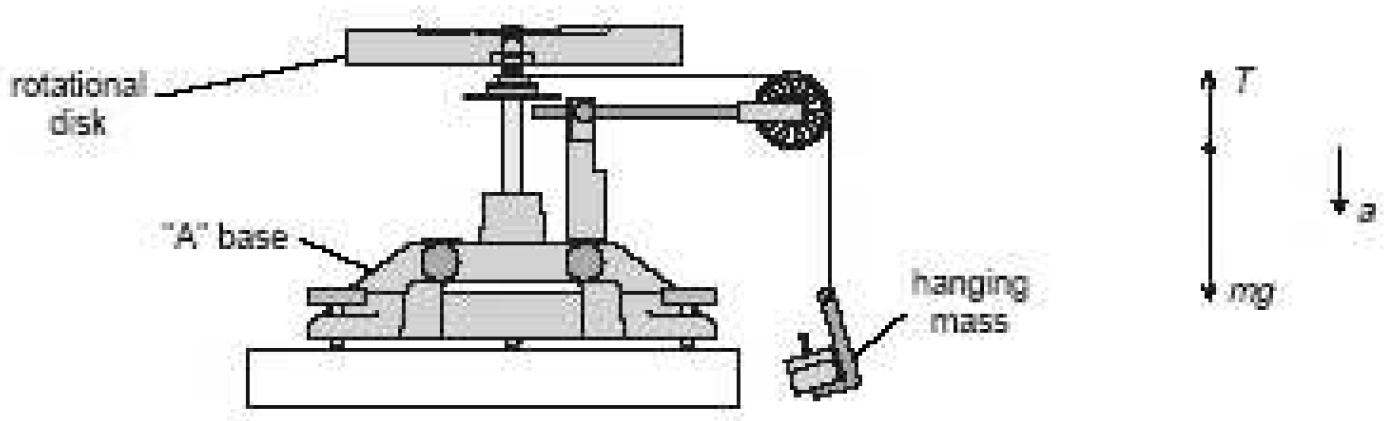
\includegraphics[width=\linewidth]{../prilohy/aparatura_1.png}
				\caption{Nákres aparatury převzatý z \cite{bib:zadani}.}
				\label{fig:s_aparatura_moment}
					    	
				
		\end{center}
	\end{figure}
	\begin{figure}[h!]
			\begin{center}
			    	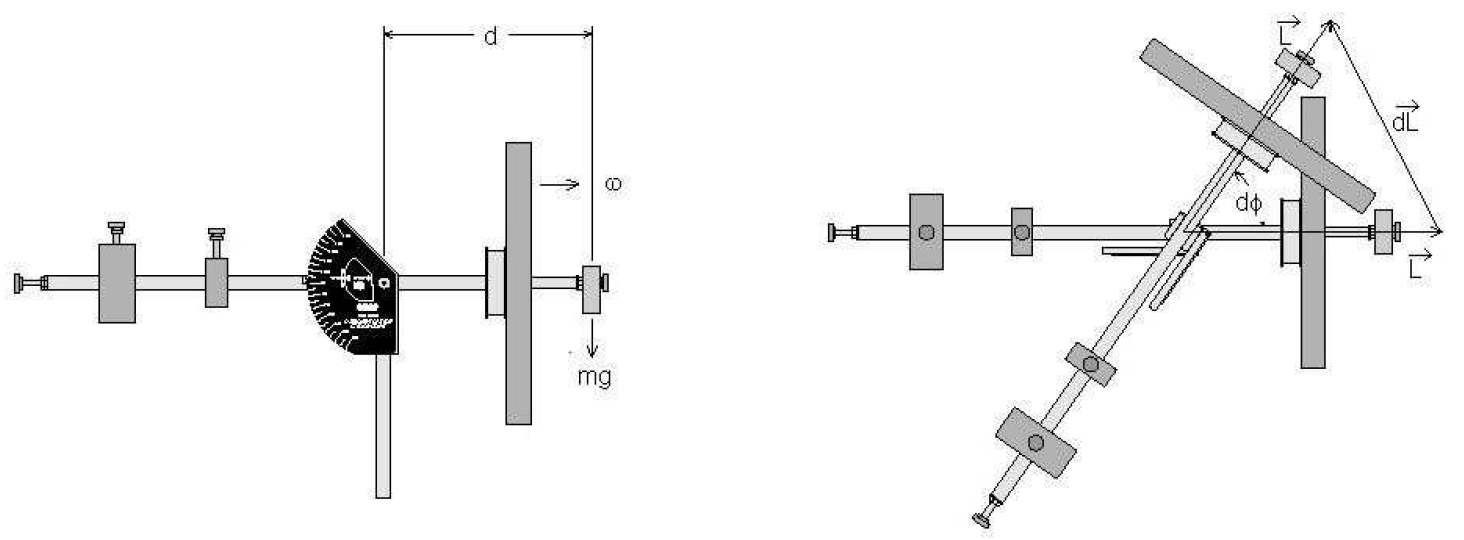
\includegraphics[width=\linewidth]{../prilohy/aparatura_2.png}
					\caption{Nákres aparatury převzatý z \cite{bib:zadani}.}
					\label{fig:s_aparatura_gyro}
						    	
					
			\end{center}
		\end{figure}	
	

\clearpage
\subsection{Grafy}

	\begin{figure}[h]
	\begin{center}
	    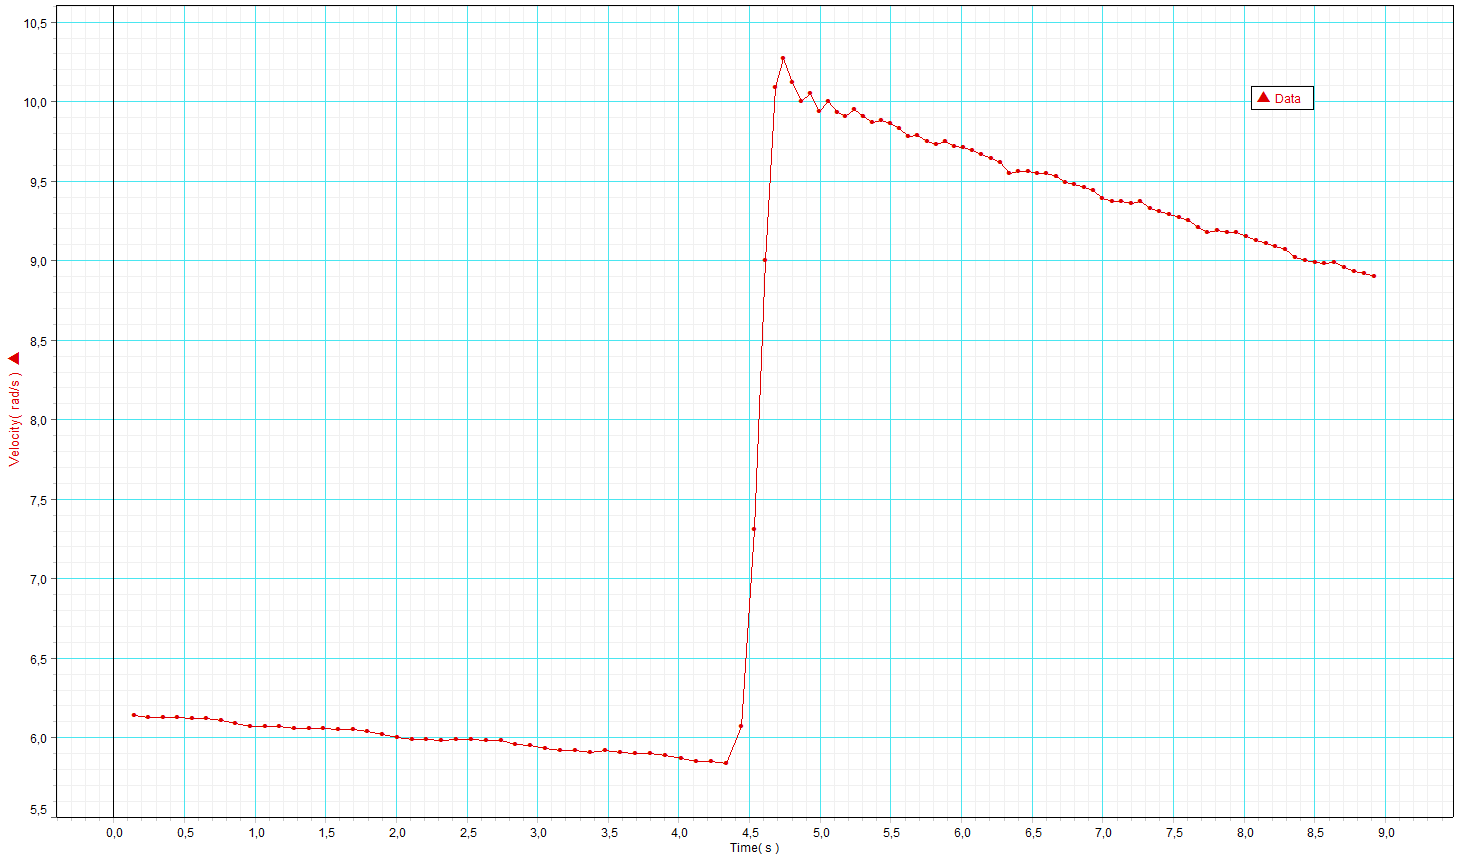
\includegraphics[width=\linewidth]{../prilohy/data.png}
	    	\caption{Graf úhlové rychlosti v závislosti na čase vyexportovaný z programu \emph{DataStudio}; \emph{Data} jsou naměřené hodnoty. Přibližně v čase $t=4,5$ s můžeme vidět zrychlení otáček způsobené přiblížením závaží k sobě.}
			\label{fig:g_zzmh}
	\end{center}
	\end{figure}
	
% --- Konec dokumentu --------------------------------------------------


\end{document}

